\newpage
\section{Лекция 14}
\subsection{Положительные и неотрицательные матрицы}
Пусть $A\in M_n(\mathbb{R})$, тогда
$$A\geqslant B \Leftrightarrow a_{ij}\geqslant b_{ij} ~~\forall i, j$$
$$A> B \Leftrightarrow a_{ij}> b_{ij} ~~\forall i, j$$
Однако не все матрицы сравнимы.\\
\\
\textbf{Пример 1.}\\ \\
\[\begin{pmatrix}[r]
2\\
1\\
\end{pmatrix}\geqslant \begin{pmatrix}[r]
1\\
1\\
\end{pmatrix}\]\\
\[\begin{pmatrix}[r]
2\\
1\\
\end{pmatrix}\neq \begin{pmatrix}[r]
1\\
1\\
\end{pmatrix}\]\\
\[\begin{pmatrix}[r]
2\\
1\\
\end{pmatrix}\ngtr \begin{pmatrix}[r]
1\\
1\\
\end{pmatrix}\]
\begin{definition}
    Матрица называется \textbf{неотрицательной}, если $A\geqslant 0$ тогда и только тогда, когда все $a_{ij}\geqslant 0$.
\end{definition}
\begin{definition}
    Матрица называется \textbf{положительной}, если $A> 0$ тогда и только тогда, когда все $a_{ij}> 0$.
\end{definition}
\begin{definition}
    \textbf{Матрица смежности} $G>0,~G\ngtr 0$ --- матрица с элементами $g_{ij}$, причем $g_{ij}=1$, если есть ребро из вершины $i$ в вершину $j$ и $g_{ij}=0$ иначе (вместо единицы может также стоять какое-либо число $k$, равное количеству ребер из вершины $i$ в $j$ или весу ребра).
\end{definition}
\begin{theorem}[Перрона]
    Если $A>0$ матрица положительная, то существует такое $\hat \lambda_A>0$ --- собственное значение матрицы $A$, что $\hat \lambda_A>|\lambda|$ для всех остальных собственных значений $A$ и соответствующий собственный вектор $\hat x$ положителен
$$A\hat x=\hat \lambda_A \hat x,~\hat x>0.$$
В частности, $$\rho_(A)=\hat \lambda_A.$$
\end{theorem}
\begin{consequence}
    Вектор $\hat x$, соответствующий $\hat \lambda_A$ единственный с точностью до пропорциональности. В частности, $\hat \lambda$ --- простое, кратности один.
\end{consequence}
\subsection{PageRank}
Есть конечное число состояний и вероятности перехода из одного состояния в другое. Какова вероятность на каком-то шаге $n$ попасть в состояние $i$? (Какова вероятность, что пользователь окажется на нашем сайте?)
$$\bar x_n=(p_1 \cdots p_i \cdots p_n)^T$$
$$P=(p_{ij}):~x_n=P^n\cdot x_0$$
Стабильным состоянием системы называется $$x_{n+1}=Px_n=x_n.$$
При $n\to \infty ~~\hat x=x_{\infty}~~Px_n=1\cdot x_n$, где собственное значение равно единице.
Не все $p_{ij}$ могут быть даны (на каких-то сайтах нет ссылок).\\
Собственный вектор $(x_1 \cdots x_n)^T$, где $x_i$ --- соответствующие вероятности попаст на какую-то страницу. Тогда первой страницей будет выдаваться страница с наибольшим собственным значением и так далее по убыванию.
$$\bar x=x_1P^1+x_2P^2+\cdots +x_NP^N$$
\\
Вместо $P$ в PageRank можно также смотреть подправленное значение $$\tilde{ P}=P(1-\beta)+\beta Q$$ Обычно берут $\beta=0.15$, а 
\[Q = \begin{pmatrix}[r]
\cfrac{1}{n} & \cdots & \cfrac{1}{n}\\
\vdots & \ddots & \vdots\\
\cfrac{1}{n} & \cdots & \cfrac{1}{n}\\
\end{pmatrix},\]
где $n$ --- количество всех страниц в интернете.\\ \\
\begin{consequence}
    Пусть $A\geqslant 0$ неотрицательная матрица, тогда
\begin{enumerate}
    \item Существует собственное значение, равное спектральному радиусу $$\exists \hat \lambda_A=\rho(A)\geqslant 0$$
    \item Собственный вектор $\hat x_A\geqslant 0$ (не обязательно единственный)
\end{enumerate}
\end{consequence}
\textbf{Пример 2.}\\
Найти самую влиятельную вершину в графе, сформировать предпочтения.\\
\begin{center}
    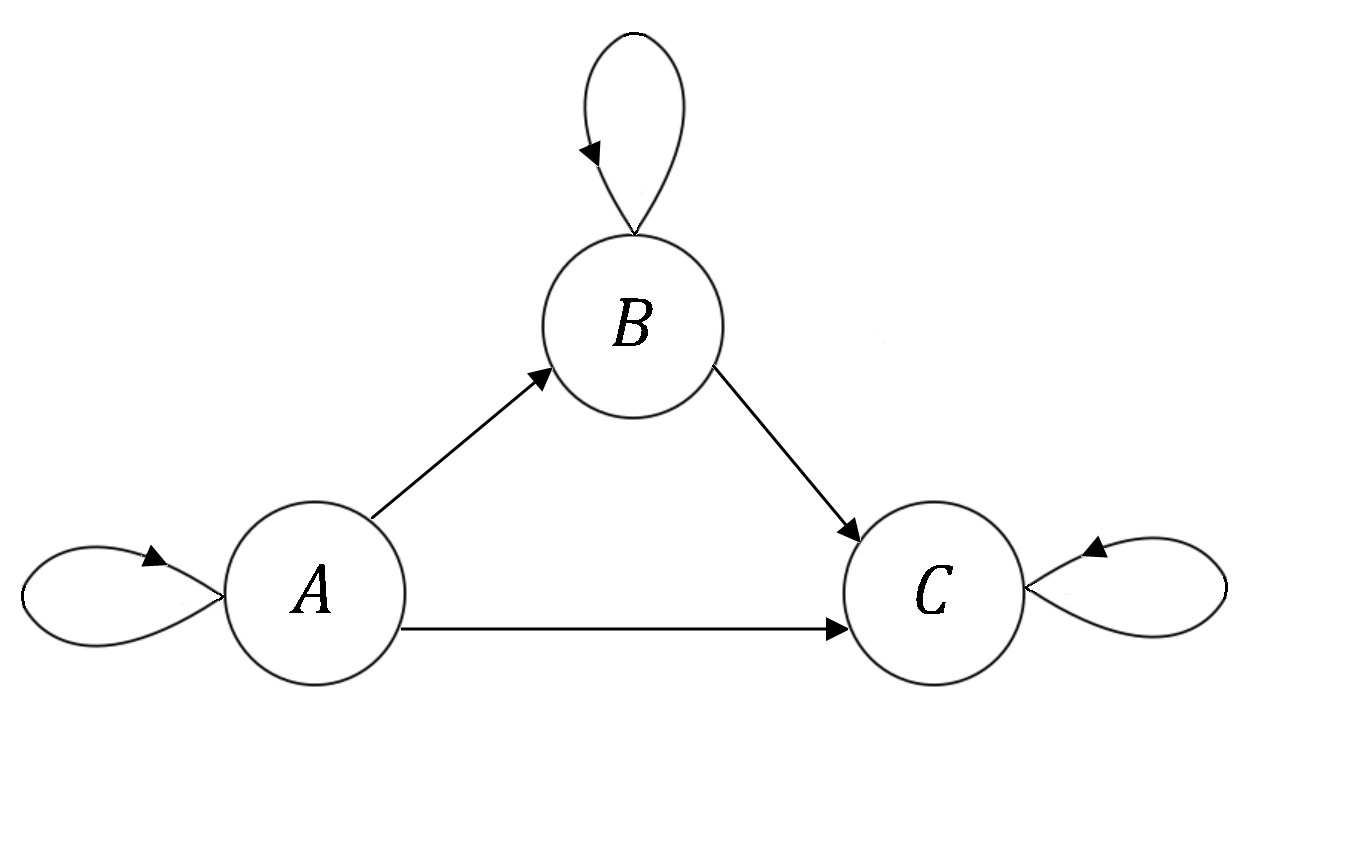
\includegraphics[scale=0.35]{l14_4.png}\\
\end{center}
Составим матрицу по графу:
\[P = \begin{pmatrix}[r]
\cfrac{1}{3} & \cfrac{1}{3} & \cfrac{1}{3}\\
0 & \cfrac{1}{2} & \cfrac{1}{2}\\
0 & 0 & 1\\
\end{pmatrix}\]
В начальном состоянии рангии равны:
\[\bar x_0 = \begin{pmatrix}[r]
\cfrac{1}{3}\\
\cfrac{1}{3}\\
\cfrac{1}{3}\\
\end{pmatrix} \approx \begin{pmatrix}[r]
0.333\\
0.333\\
0.333\\
\end{pmatrix} \approx \begin{pmatrix}[r]
0\\
0\\
0\\
\end{pmatrix}\]
Вычислим дальше:
\[\bar x_1 = P^T\bar x_0=\begin{pmatrix}[r]
\cfrac{1}{3} & 0 & 0\\
\cfrac{1}{3} & \cfrac{1}{2} & 0\\
\cfrac{1}{3} & \cfrac{1}{2} & 1\\
\end{pmatrix}\bar x_0 = \begin{pmatrix}[r]
\cfrac{1}{9}\\
\cfrac{5}{18}\\
\cfrac{11}{18}\\
\end{pmatrix} \approx \begin{pmatrix}[r]
0.111\\
0.277\\
0.611\\
\end{pmatrix}\approx \begin{pmatrix}[r]
0\\
0\\
1\\
\end{pmatrix}\]
\[\bar x_2 = P^T\bar x_1= \begin{pmatrix}[r]
\cfrac{1}{27}\\
\cfrac{19}{108}\\
\cfrac{85}{108}\\
\end{pmatrix} \approx \begin{pmatrix}[r]
0.037\\
0.175\\
0.787\\
\end{pmatrix}\approx \begin{pmatrix}[r]
0\\
0\\
1\\
\end{pmatrix}\]
Таким образом, получили ранги:
$$C=1,~~A=B=0,$$
значит самая влиятельная вершина в графе это $C$.
\begin{definition}
    Матрица $A$ называется \textbf{неразложимой матрицей}, если одновременно перестановкой строк и столбцов матрицу $A$ нельзя привести к виду
\[ 
A=
\left(
\begin{BMAT}[8pt]{c:c}{c:c}
P & Q\\
O & R\\
\end{BMAT} 
\right),
\]
где $P$ и $R$ --- квадратные матрицы, а $O$ --- нулевая матрица.
\end{definition}
\begin{theorem}[Перрона Фробениуса]
    Пусть $A\geqslant 0$ и $A$ --- неразложимая матрица, тогда $\hat \lambda_A>0$ и $\hat x>0$ --- единственный с точностью до множителя.
\end{theorem}
\subsection{Модель Леонтьева и продуктивные матрицы}
Есть несколько отраслей и несколько категорий продукций. Матрица Леонтьева имеет вид:
\[ 
\begin{BMAT}[8pt]{|c|cccc|}{|c|cccc|}
o~|~p & 1 & 2 & \cdots & n\\
1 & a_{11} & a_{12}& \cdots & a_{1n}\\
2 & a_{21} & a_{22} &\cdots & a_{2n}\\
\vdots & \vdots  &\cdots &\ddots & \vdots\\
m      & a_{m_1}  &\cdots &\cdots &a_{mn}\\
\end{BMAT} 
\]
$$A\bar x+\bar d=\bar x$$
$A=(a_{ij})$, где $a_{ij}$ --- количество продукции $j$ в отрасли $i$ для производства (матрица прямых затрат), $d$ --- конечный спрос, а $x$ --- выпуск.
Продукция отрасли $i$: $$x_i=d_i+\sum\limits_j a_{ij}x_j,$$
первое слагаемое означает употребление, а второе --- использование для производства.\\
\begin{definition}
    Матрица $A$ называется \textbf{продуктивной}, если $A\geqslant 0$ и для некоторого $\bar x > \bar 0$ верно $$A\bar x <\bar x.$$
\end{definition}
Если $A\geqslant 0,~B\geqslant 0$, то $A-B=(c_{ij})$, где $c_{ij}=\sum\limits_k a_{ik}b_{kj}\geqslant 0,~c\geqslant 0$.
\begin{lemma}
    \ 
    \begin{enumerate}
        \item Если матрица неотрицательная $A\geqslant 0$ и $x_1 \geqslant x_2$, то $Ax_1 \geqslant Ax_2$.
        \item Если матрица $A$ продуктивная, то $\underset{n\to \infty}{lim}A^n=0$.
        \item Если матрица $A$ --- продуктивная и для какого-то $\bar y$
        $$\bar y \geqslant A\bar y,$$ то $\bar y$ --- неотрицательный вектор.
    \end{enumerate}
\end{lemma}
\begin{proof}
    \ 
    \begin{enumerate}
        \item Надо проверить $Ax_1-Ax_2 \overset{?}{\geqslant} 0$.\\
        $$A(x_1-x_2)\geqslant 0,$$
        так как $A\geqslant 0$ и $x_1-x_2 \geqslant 0.$
        \item По определению продуктивной матрицы $A\bar x< \bar x$, тогда существует число $0<\alpha <1$, где $\alpha$ --- константа сжатия, что:
        $$Ax<\alpha x$$
        $$0\leqslant A^n x<\alpha^n x$$
        При $n\to \infty$ $\alpha \to 0$, тогда получим $\underset{n\to \infty}{lim}A^nx=0$, тогда $\underset{n\to \infty}{lim}A^n=0$, так как $x$ --- положительный вектор.\\
        Подробнее: если $A^n=(b_{ij})$, то 
        \[A^n \bar x = \begin{pmatrix}[r]
        \sum\limits_{j=1}^n b_{1j}x_j\\
        \vdots\\
        \sum\limits_{j=1}^n b_{nj}x_j\\
        \end{pmatrix}=\bar 0,\]
        где $x_j>0,~ b_{ij}\geqslant 0$. Значит все $b_{ij}=0,~A^{\infty}=0$ по первой части леммы.
        \item Будем подставлять $y$ в наше условие много раз: $$y\geqslant Ay \geqslant A^2y \geqslant \cdots \geqslant A^n y \geqslant \cdots \geqslant A^{\infty} y =\bar 0$$ по лемме 2, значит $\bar y \geqslant 0.$
    \end{enumerate}
\end{proof}
\begin{theorem}
    Пусть $M$ --- полное метрическое пространство (например, $M=\textbf{R}^n$ или $M \subset \textbf{R}^n$ --- замкнутое ограниченное множество), $f:~M\to M$ --- сжимающее, то есть существует $0<\alpha <1$ такое, что для $\forall x, y \in M$
$$\rho(f(x), f(y))\leqslant \alpha \rho(x, y),$$
тогда существует единственная неподвижная точка --- такое $z\in M$, что $f(z)=z$.\\
\begin{center}
    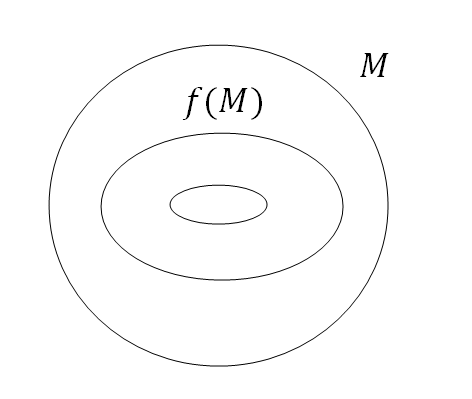
\includegraphics[scale=0.7]{l14_1.png}\\
\end{center}
$M$ отображается в $f(M)$ и так далее. В пределе диаметр стремится к нулю.
\end{theorem}
\begin{lemma}
    Если матрица $A$ --- продуктивная, то существует $(E-A)^{-1}\geqslant 0$. (А если $A>0$, то $(E-A)^{-1}$ положительная матрица.)
    
    Как следствие, если $A\geqslant 0$ --- неразложимая и продуктивная матрица, то $(E-A)^{-1}>0$.
\end{lemma}
\begin{proof}
    $(E-A)^{-1}=E+A+A^2+\cdots +A^n+\cdots$ --- ряд сходится, так как $A^n \to 0$, тогда $\rho(A)<1$ и так далее.\\
$$(E-A)^{-1}\geqslant E+A \geqslant A$$
Если $A>0$, то $(E-A)^{-1}>0$, а если $A\geqslant 0$, то $(E-A)^{-1}\geqslant 0$
\end{proof}
\begin{theorem}
    Если $A$ --- продуктивная, то для любого $\bar d \geqslant \bar 0$ система $A\bar x+\bar d=\bar x$ имеет единственное решение $\bar x$, причем $\bar x \geqslant 0$.
\end{theorem}
\begin{proof}
    Выразим $x-Ax=d$ или $(E-A)\bar x=\bar d$. Так как матрица $A$ продуктивная из леммы 4 и следствия выше получим $\bar x=(E-A)^{-1}\bar d\geqslant 0$
\end{proof}
\begin{consequence}
    Для $d>0$ система имеет решение $x \geqslant 0$ тогда и только тогда, когда матрица $A$ продуктивная.
\end{consequence}
\begin{proof}
    Если $(E-A)\bar x=\bar d,~\bar d>0$, то $x=Ax+d>0$, причем $x>Ax$, а это по определению означает, что матрица $A$ продуктивная.
\end{proof}
\begin{statement}
    \ 
\begin{enumerate}
    \item Матрица $A$ является неразложимой тогда и только тогда, когда для $\forall i, j, i\neq j$ существует такая последовательность вершин $$i=i_0, i_1, i_2, \cdots, i_k=j:~~a_{i_t i_{t+1}}\neq 0,~t=0, \cdots, k-1$$
    \begin{center}
        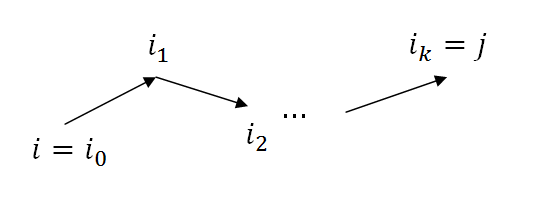
\includegraphics[scale=0.6]{l14_2.png}\\
    \end{center}
    \item Матрица $A$ неразложима тогда и только тогда, когда для любых вершин $\forall i, j$ существует $\exists m<n$, что $$(A^m)_{ij}\neq 0.$$
    \item Неотрицательная матрица $A\geqslant 0$ неразложима тогда и только, когда $(E+A)^{n-1}>0$, где $n$ --- порядок матрицы.
\end{enumerate}
\end{statement}
\begin{proof}
    \ 
    \begin{enumerate}
    \item Матрица $A$ является разложимой тогда и только тогда, когда существует $\exists S=\{i_1,\cdots, i_s\} \subsetneq [1, \cdots, n]$. Тогда $a_{ij}=0$ при $j\in S,~i\notin S$, где $1\leqslant |S| \leqslant n-1$.\\
    \begin{center}
        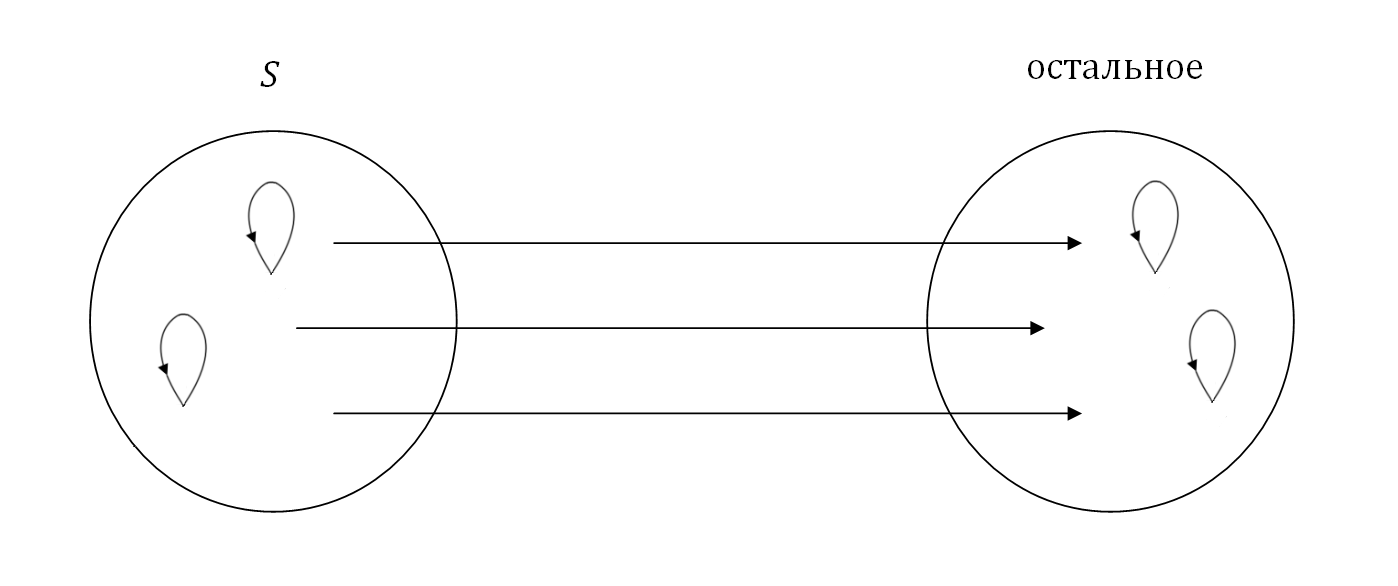
\includegraphics[scale=0.6]{l14_3.png}\\
    \end{center}
    (Можем перенумеровать индексы.)\\
    Стрелка $i\to j$ существует тогда и только тогда, когда $a_{ij}\neq 0$.\\
    В разложимой матрице какого-то пути нет, в неразложимой матрице все пути есть.
    \item $a_{ij}$ равно количеству путей $i\to j$ длины один, а $(A^m)_{ij}$ равно количеству путей $i\to i_1\to \cdots i_{m-1}$ длины $m$.
    \item Путь длины $n-1$ $(E+A)^{n-1}=\sum\limits_{m=0}^{n-1}C_{n-1}^mA^m>0$, так как в каком-то слагаемом будет ненулевой элемент, то есть получим положительное число. 
\end{enumerate}
\end{proof}
\subsection{Домашнее задание 14}\begin{enumerate}
    \item Найти самую влиятельную вершину в графе.
    \begin{center}
        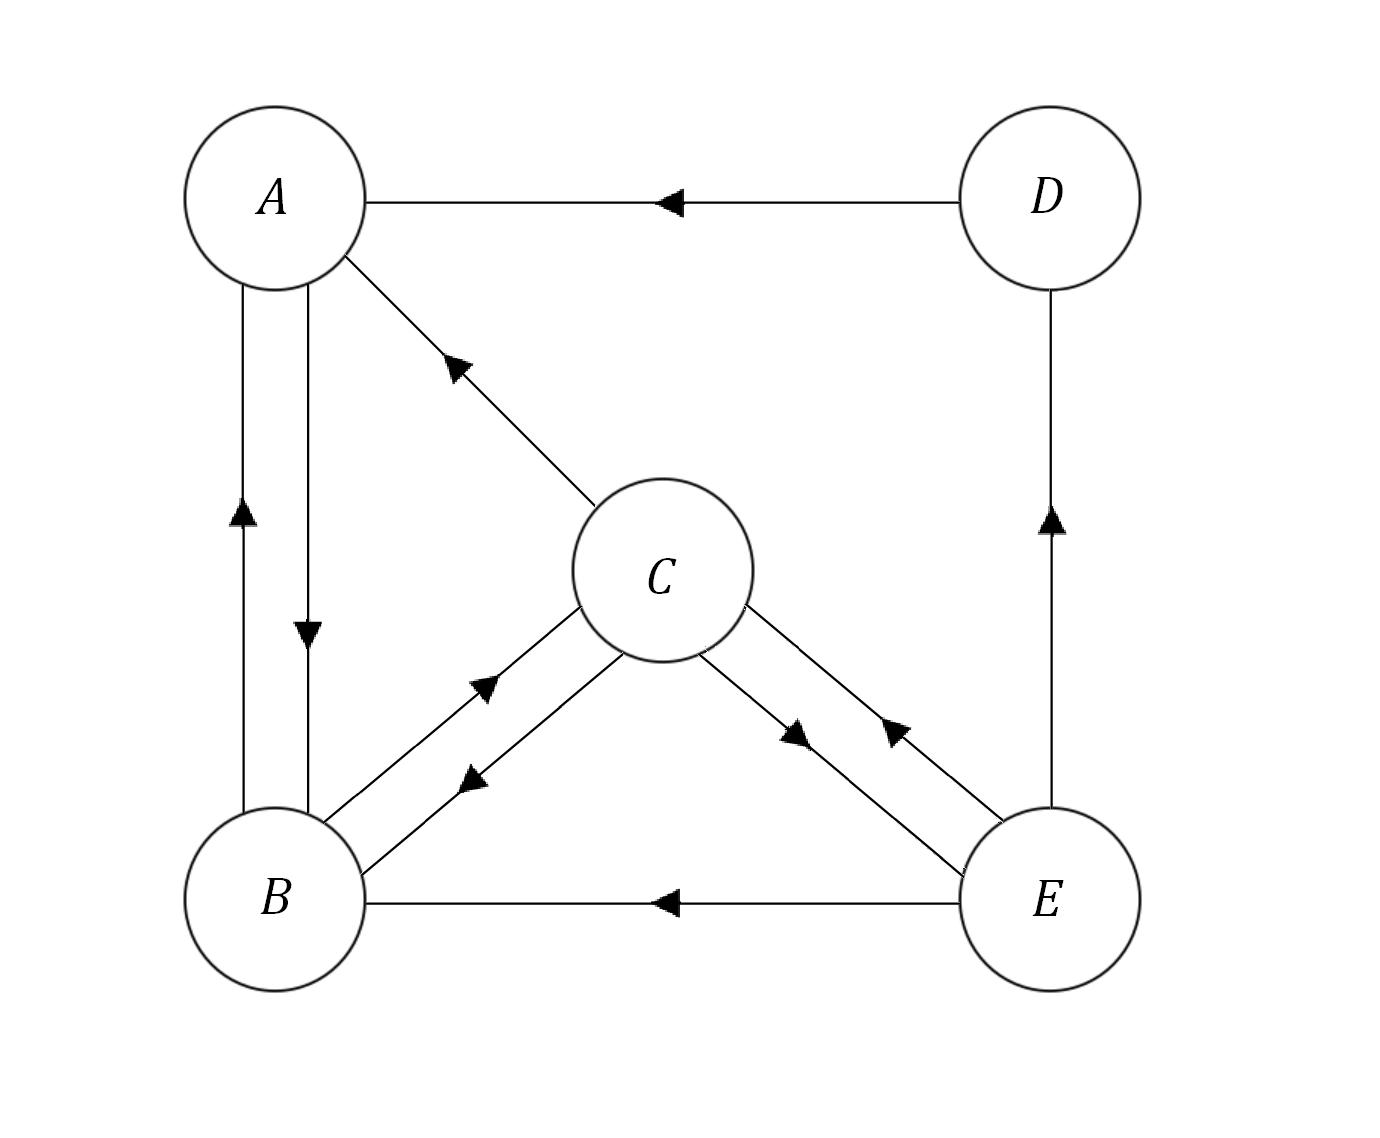
\includegraphics[scale=0.35]{l14_5_.png}\\
    \end{center}
    \item Разложима ли матрица $A$?
    \[A = \begin{pmatrix}[r]
    0 & 1 & 2 & 0 & 0\\
    0 & 0 & 0 & 7 & 0\\
    2 & 0 & 0 & 0 & 0\\
    0 & 9 & 2 & 0 & 4\\
    0 & 0 & 0 & 1 & 0\\
    \end{pmatrix}\]
    \item Разложима ли матрица $B$? Найти $\lambda$ и $v$ из теоремы Перрона.
    \[B = \begin{pmatrix}[r]
    0 & 1 & 0\\
    3 & 0 & 3\\
    0 & 2 & 0\\
    \end{pmatrix}\]
\end{enumerate}
